\documentclass{article}
\usepackage{verbatim}
\usepackage{amssymb}
\usepackage{fullpage}
\usepackage{float}
\usepackage{algorithmicx}
\usepackage{graphicx}

\usepackage[english]{babel}
\usepackage[utf8]{inputenc}
\usepackage{algorithm}
\usepackage[noend]{algpseudocode}

\newcommand\eqdist{\mathrel{\stackrel{\makebox[0pt]{\mbox{\normalfont\tiny d}}}{=}}}



\graphicspath{{figs/}}
%\author{Lucas Roberts}
%\date{\today}
\begin{document}
\title{
Why nematologists should use zero-inflated models when modeling count data. (And how to use them)
}

\maketitle

\section{Introduction}
Counts of nematodes, abundance measures, and rates within a unit volume of soil are all common count measures of nematodes. The method of counting after elutriation is time consuming but conceptually straightforward for the researcher. In our own work \cite{} we have found count models of nematodes as well as root count measures in vineyards to be inadequate statistical models in most observed data. The count data are often observed with a high prevalence of zeroes, indeed often beyond the frequency of zeroes suggested by the Poisson model itself. In cases with excess zeroes the use of a Poisson model is inadequate to describe the data. Zero-inflated models offer an alternative that accounts for the excess zeroes observed as well as providing additional over dispersion flexibility. Recall, a distribution is called over-dispersed if the variance exceeds the mean, $\sigma^2 > \mu$. 

In many cases nematologists, and scientists in general use the Poisson model not because it is appropriate for the observed data but because the scientist is familiar with the modeling approach of calculating sample means. This article is meant to bring the zero-inflated models to the attention of scientists modeling count data and point out the pitfalls of using traditional methods in the presence of excess zero counts. The use of zero inflated models is common in other scientific disciplines such as (cite list\cite{}) and has been seen in the analysis of nematode count data by Murray et al. \cite{murray2011modeling}. Murray mention that the zero-inflation might come not from the lack of nematodes but from the symbiotic relation certain species of nematodes have with the root system, once the nematode embeds in the root system there is no ability to measure the organism. The only time the organism may be measured is when recently-hatched pre-parasitic second stage juveniles (SRKN-J2) are detectable in soil prior to host invasion.

There are readily available software for fitting zero-inflated models. We provide a table of common statistical software to fit zero-inflated models and compare relevant aspects of these software. Moreover, for the scientist who prefers to `cook their own' statistics we also provide a spreadsheet in an appendix at the publisher's website so that the scientist may perform the calculations on simplified zero-inflated Poisson models themselves. Also the spreadsheet serves as an instructional aid, the scientist may study the formulae and calculations to ensure their understanding of the model and resulting calculations.  

Beyond the statistical aspects of zero-inflated models of count data there are very important scientific considerations for using these models, not the least of which is that the failure to use zero-inflated models when the data are in fact zero-inflated leads to bias in the reported rates of nematodes per unit volume of soil. The reported rate estimates under the traditional models will be underestimated and may cause a grower to fail to act when in fact the should make efforts to control their nematode population by perhaps cleansing field tools before moving from one area to another in the field and other mitigation methods beyond methyl bromide outlined by Zasada et al. \cite{zasada2010managing}.  Additionally, the scientist might think that as long as they collect a sufficient number of samples the bias from mis-specifying the Poisson model will be negligible, we show this is not the case and in fact the larger the underlying rate of nematodes the larger the error in estimation. 

\begin{itemize}
\item Models encompass traditional count data models as special cases and account for excess zeros common in nematology. 
\item Readily available-and often free-software has ready made codes to fit zero-inflated models. 
\item Using Poisson based models when zero-inflation is present leads to biased estimates and larger mean squared errors.   
\end{itemize}

\section{Estimation challenges}

The Bias of an estimator is defined as the expected value of the estimator minus the parameter to be estimated. In the case of count data often the researcher wants to know the rate parameter which indicates an average number of nematodes per unit of soil volume. Let the rate parameter be denoted $\lambda$ and the zero inflation probability be denoted $\phi$. If the researchers use the common average of the count data, denoted $\bar{y}$, then under a ZIP distribution the expected value of this estimator is 

\begin{equation}
\mathbb{E}(\bar{y}) = (1-\phi)\lambda.
\end{equation}
Thus the bias of the estimate is 

\begin{equation}
\underbrace{\mathbb{E}(\bar{y}) - \lambda}_{=bias} = -\phi\lambda,
\end{equation}
so that the larger the zero-inflation or the rate parameter, the larger the bias of the estimate. 

One common approach to handle excess zeroes in count data is to add 1 to each observed count. If the counts are indeed Poisson distributed, the resultant random variable is a size-biased Poisson \cite{arratia2013size,arratia2010size}. Regardless of the underlying distribution the rate estimate will now be biased by 1. To remove this bias you may safely subtract 1 from the average. Note this does not solve the problem of excess zeroes. Another common method especially when analyzing abundance data (e.g. \cite{jagdale2013incidence}) is to condition on the count being greater than zero  which is equivalent to ignoring the zero counts. Under a ZIP distribution one case show that this distribution $\Pr(Y=y \vert y>0)$ has a zero-truncated Poisson distribution. For more on the statistical properties of this distribution see Cohen \cite{cohen1960estimating} and Singh \cite{singh1978characterization}. Unfortunately the sample mean is not an unbiased estimate of the rate parameter $\lambda$ in the zero-truncated case either. Moreover, some authors prefer to use a transformed version of the count with a 1 added, some examples are $log(y+1)$ \cite{howland2014spatial,centinari2016root} or $\sqrt{2(y+1)}$ \cite{anscombe1948transformation,yu2009variance}. Both lead to biased estimators of the underlying rate. The second transform which uses a squared root, has roots in the variance stabilization literature \cite{freeman1950transformations} and would be reasonable without the addition of a 1 only if the underlying counts are Poisson distributed.  

One common measure of the closeness of an estimator to a parameter is the mean squared error (MSE). The MSE is defined as the expected value of the square of the difference between the estimator and the true value of the parameter. Formally, write 
\begin{equation}
MSE(\bar{y}, \lambda) = \mathbb{E}(\bar{y}-\lambda)^2,
\end{equation}
For the average as an estimator of the rate the MSE is 
\begin{equation}
MSE(\bar{y}, \lambda) = \phi^2\lambda^2 + \frac{ \lambda(1-\phi) +\lambda^2(1-\phi)\phi}{n}.
\end{equation}
This last equation tells us that even with an infinite number of samples ($n \to \infty$) unless the zero-inflation is non-existent, there will be a bias proportional to the rate and the traditional methods will be suboptimal to use in place of estimators of zero-inflated data generating processes. The preceding portion of this section has discussed the statistical estimation of rates for data which are truly zero-inflated, in practice we never know for certain whether the data is truly zero-inflated or not and we must rely on statistical tests to make this determination. The next section discusses the methods to use to make this determination as well as the statistical nuances of these procedures.
 
\section{Model determination: Poisson or ZIP?}
There are two commonly used methods to determine whether the count data you are modeling is from a zero-inflated distribution or not: the likelihood ratio (LR) test and the Vuong test \cite{vuong1989likelihood}.  
There is a fair amount of disagreement within the scholarly community about when to use the Vuong test or the LR test \cite{wilson2015misuse}. Notwithstanding these disputes, the Vuong test is actually a class of tests that are appropriate when comparing two zero-inflated regression models that may or may not be nested. We will not detail the Vuong test for reasons of scope but the interested reader is referred to the paper by Vuong (cited above)) as well as the two econometrics textbooks \cite{2005estimation,davidson1995estimation}. The likelihood ratio test method is appropriate when comparing a Poisson model against a zero-inflated model. We will first discuss the likelihood ratio test and then the Vuong test. 

The likelihood ratio (LR) test statistic is constructed by taking twice the logarithm of the ratio of the likelihood under the unconstrained model to the likelihood under the model constrained by the null hypothesis. The standard results in statistics, applying a second order taylor series and taking limits, implies that this statistic will be asymptotically distributed as a chi-squared distribution. In our case of making a determination between a model with and one without zero-inflation the likelihood ratio test will not converge to the standard distribution in the statistical literature because the zero-inflation parameter lies on the boundary ($\phi=0$) of the parameter space \cite{chernoff1954distribution,feng1992statistical,self1987asymptotic}. The case when the likelihood ratio statistic has a parameter on the boundary of the parameter space is a well studied and understood problem within statistics that occurs in other models as well, such as a mixed effect model when you want to test whether one of the variance components is 0 or not \cite{crainiceanu2004likelihood}. The traditional results state that the distribution of the LR test statistic has a point mass mixture distribution with probability one-half at the zero point and then other half is spread over a chi-squared distribution with a single degree of freedom. Formally twice the log-likelihood random variable, denoted $\xi$ is distributed 

\begin{equation}
\xi \eqdist \frac{\chi^2_0}{2} + \frac{\chi^2_1}{2},
\end{equation}
where the zero degree of freedom chi-squared random variable is interpreted as a point mass at zero. To illustrate this phenomena to the reader we generate Figure \ref{fig:twice_log_likelihood} which displays the results of $10,000$ random draws from a zero-inflated Poisson distribution with $\phi=0.36788$ and rate parameter $\lambda=1$. 
We form the LR test statistic by comparing a Poisson likelihood and a zero-inflated Poisson likelihood and taking twice the logarithm of the difference of the two. The bold line displays the  theoretical distribution which contains a point mass at zero and a chi-squared density on the positive axis. This has implications for the nematologist who is testing whether to use a ZIP model versus a Poisson model, the test statistic p-value may be calculated exactly by calculating one-half the upper tail of a chi-squared distribution with 1 degree of freedom, unless the LR test statistic is zero in which case the p-value is 1. Table \ref{tab:table1} gives the critical values of the distribution for various common type 1 error rates. 

\begin{figure}[H]
\label{fig:twice_log_likelihood}
\vspace{0.5in}
\begin{center}
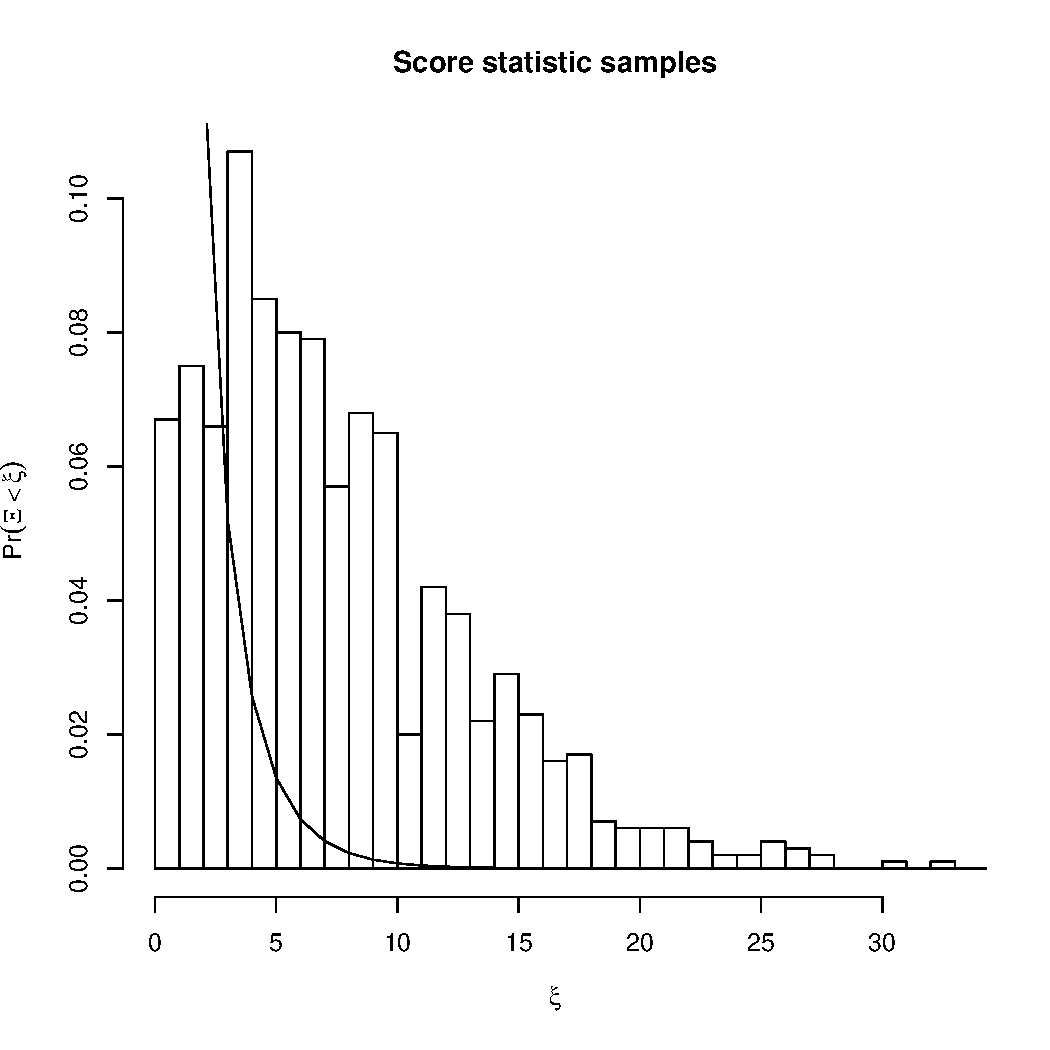
\includegraphics[scale=0.6]{hist.pdf}
\end{center}
\end{figure}

\begin{table}
 \label{tab:table1}
\begin{center}
\begin{tabular}{llr}
\hline
\multicolumn{2}{c}{Likelihood ratio test} \\
\cline{1-2}
P-value & Critical value $\xi$ \\
\hline
0.001 & 9.549536\\
0.01 &5.411894 \\
0.025 &3.841459\\
0.05 &2.705543\\
0.1 &1.642374\\
0.25 & 0.454936\\
\hline
\end{tabular}
\end{center}
\caption{The critical values of the likelihood ratio test. }
\end{table}

\section{An algorithm for estimating $\phi$ and $\lambda$ with no covariates}

In this section we detail an algorithm for estimating the two parameters of a ZIP model that is readily programmable within a spreadsheet with basic arithmetic calculations. Although the algorithm contains a while loop that is potentially infinite, in our experience the number of iterations is typically no more than 5-10. Moreover, the calculations required in each iteration are readily programmed so that the researcher may apply the technique to various data via copy and paste to mimic the iterations of the while loop. The algorithm follows: 

\begin{algorithm}
\caption{ZIP EM algorithm}\label{alg:zip_em}
\begin{algorithmic}[1]
\Procedure{ZIP EM}{$\phi^0,\lambda^0, \varepsilon, \vec{y}, \vec{w}$}
\For{$i \gets 1, n$}
 	\If{$y_i =0$}
  		\State $w_i \gets (1+\exp[-\lambda_i^0 -\textnormal{log}(\phi_i^0/(1-\phi_i^0))])^{-1}$ 
	\Else 
  		\State $w_i \gets 0$ 
 	\EndIf
\EndFor
\State $t \gets 1$
\While{$\varepsilon > \vert\phi^t - \phi ^{t-1}\vert$ and $\varepsilon > \vert\lambda^t - \lambda^{t-1}\vert$}
\State $\phi^t \gets \sum_{i=1}^nw_i/n $\\
\State $\lambda^t \gets \sum_{i=1}^n(1-w_i)y_i /(\sum_{i=1}^n1-w_i) $\\
\For{$i \gets 1, n$}
 	\If{$y_i =0$}
  		\State $w_i \gets (1+\exp[-\lambda_i^t -\textnormal{log}(\phi_i^t/(1-\phi_i^t))])^{-1}$ 
	\Else 
  		\State $w_i \gets 0$ 
 	\EndIf
\EndFor

\State $t\gets t+1$\\
\EndWhile
\State \textbf{return} $\phi^t, \lambda^t$\Comment{The EM algorithm (MLE) estimates}\\
\EndProcedure
\end{algorithmic}
\end{algorithm}
The Algorithmic description is a formal way of stating the algorithm which in essence involves iterating the calculations on lines 9 and 11 and update after an initialization. For initial values of $\phi^0, \lambda^0$, and $\vec{z}$ I suggest random uniform numbers between 0 and 1 for all three. Note that all final values output by the algorithm (e.g $z_i$ and $\phi^t$) will be between 0 and 1 except for $\lambda^t$ which may be any positive value. Although a while loop is formally used in the algorithm often iterating for $t=10$ is sufficient for reasonable settings of numerical accuracy. 

A spreadsheet to accompany the manuscript is available to illustrate the necessary calculations as well as provide a working template for the nematologist. The spreadsheet is titled \texttt{phi\_lambda\_calc.xlsx} and is available in the supplementary material on the journal website. 

\section{Discussion}
In this brief research note we discussed the zero-inflated distributions and several statistical and scientific implications of nematodes using the standard statistical techniques when modeling nematode abundance with count data. We argue that all nematologists should be familiar with zero-inflated models and use these methods in place of the standard classical statistics to estimate rates of nematodes in soil volume data. For the researcher to determine whether a Poisson model and a ZIP model should be preferred, we  provided both likelihood ratio and the Vuong tests. The Vuong test should be used when trying to determine between two competing ZIP models with non-nested covariate structure. Moreover we stressed the computational aspects of these methods as well as the statistical nuances of the methods. Finally we provided an algorithm to estimate the rate of nematodes under a zero-inflated model and the zero-inflation probability component as well as provided a spreadsheet with calculations ready programmed for the researcher to modify as needed for their nematode abundance data. 


\bibliographystyle{plain}   % this means that the order of references
			    % is dtermined by the order in which the
			    % \cite and \nocite commands appear
\bibliography{bib} 


\end{document}
